\chapter{数据分析}

\def\la{\langle}
\def\ra{\rangle}
\cite{Abbott2020} (翻译见 \texttt{others/data\_{}analysis/}). \cite{Maggiore2014}, \cite{Jaranowski2012,Jaranowski2009}, \cite{Finn1992}.

\section{主要步骤}

\begin{figure}[htbp]
    \centering
    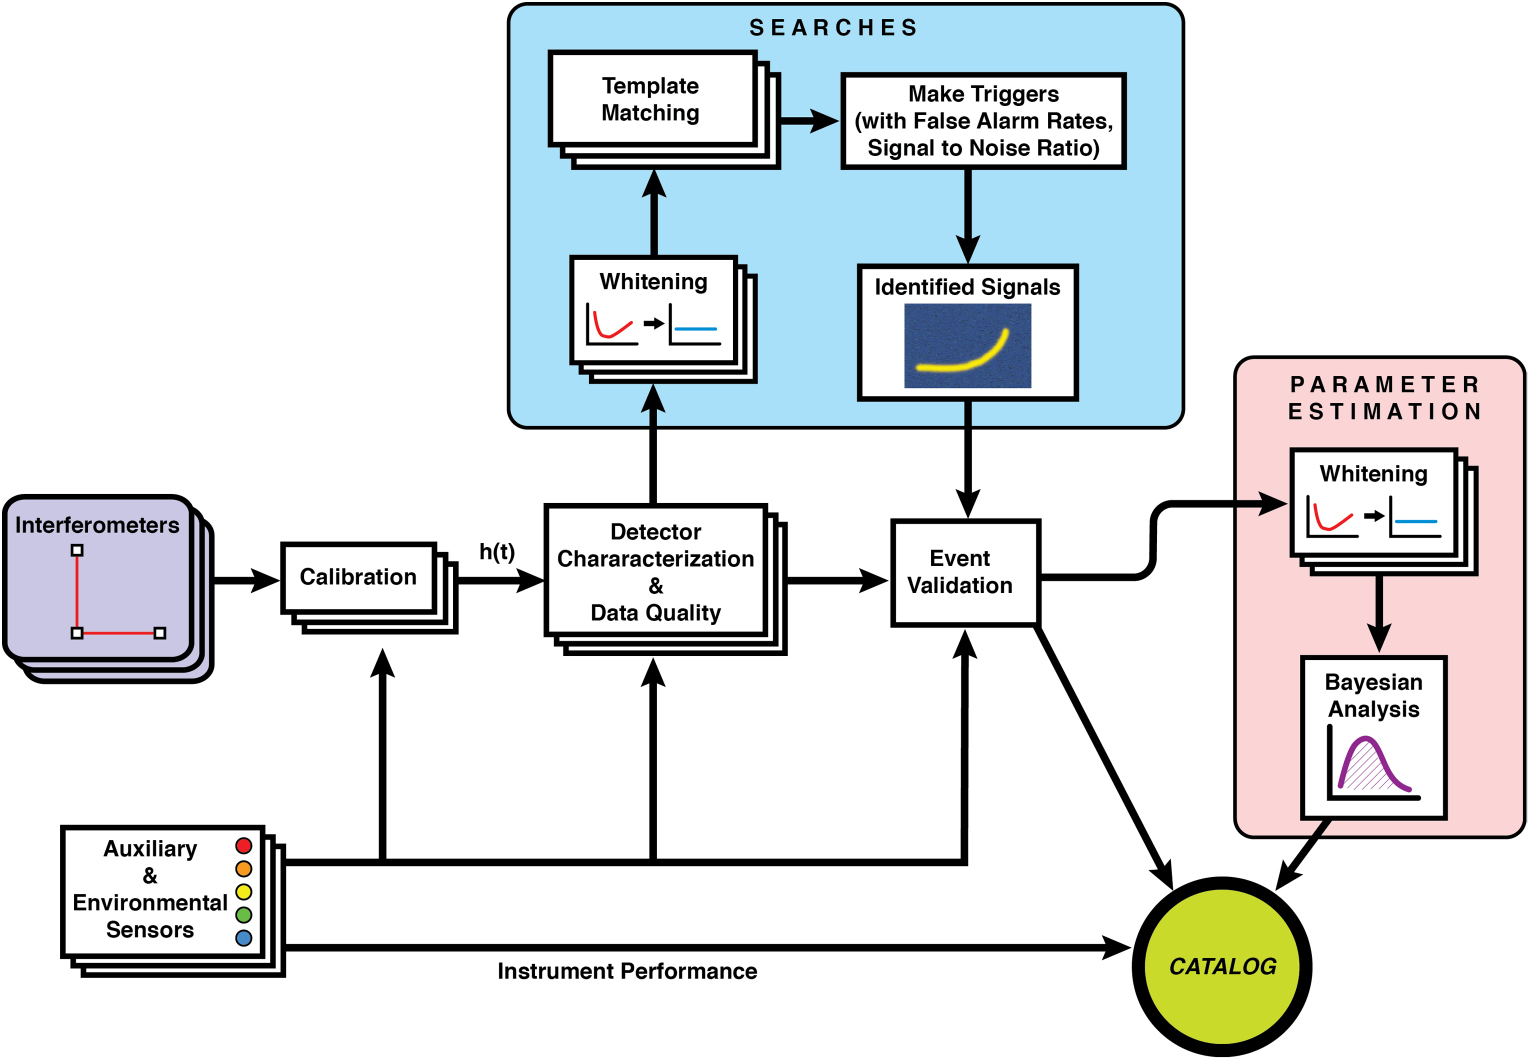
\includegraphics[width=\textwidth]{image/data_processing_main_steps.jpg}
    \caption{
        一个简化的示意图, 总结 LIGO-Virgo 数据处理的主要步骤, 从数据输出到瞬态事件表中报告的结果. 
    }
\end{figure}

\section{定义}

\begin{equation}
    R(\tau):=\text{E}(N_tN_{t+\tau}),
\end{equation}
\begin{equation}
    \frac{1}{2}S_{N}(f):=\tilde{R}(f):=\int R(\tau)e^{i2\pi f\tau}\,\d\tau.
\end{equation}
\begin{equation}
    \la p|q \ra:=4\text{Re}\int_0^\infty\frac{\tilde{p}^*(f)\tilde{q}(f)}{S_{N}(f)}\,\d f.
\end{equation}

\section{matched filtering}

\begin{equation}
    \hat{\mathcal{S}}:=\int S_tK(t)\,\d t
\end{equation}
\begin{align}
    \frac{\mathcal{S}}{\mathcal{N}}&:=\frac{\text{E}(\int (h(t)+N_t)K(t)\,\d t)}{\sqrt{\text{D}(\int N_tK(t)\,\d t)}}\\
    &=\frac{\int h(t)K(t)\,\d t}{\sqrt{\int \text{E}(N_{t_1}N_{t_2})K(t_1)K(t_2)\,\d t_1\d t_2}}\\
    &=\frac{\int h(t)K(t)\,\d t}{\sqrt{\int R(t_2-t_1)K(t_1)K(t_2)\,\d t_1\d t_2}}\\
    &=\frac{\int \ti{h}(f)\ti{K}^*(f)\,\d f}{\sqrt{\int\frac{1}{2}S_{N}(f)\ti{K}(f)\ti{K}^*(f)\,\d f}}\\
    &=\frac{\la \frac{1}{2}S_{N}\ti{K}|h \ra}{\la \frac{1}{2}S_{N}\ti{K}|\frac{1}{2}S_{N}\ti{K} \ra^{1/2}}
\end{align}
\begin{equation}
    \max{(\frac{\mathcal{S}}{\mathcal{N}})}=\la h|h \ra^{1/2}
\end{equation}

\section{parameter estimation}

\begin{equation}
    p(\mu|d)\propto p(\mu)\exp\left[-\frac{1}{2}\sum_{m,n}C_{mn}^{-1}(d_m-h_m)(d_n-h_n)\right],
\end{equation}
\begin{equation}
    p(\mu|d)\propto p(\mu)\exp\left[-\frac{1}{2}\la d-h|d-h \ra\right].
\end{equation}

\section{sensitivity}

\begin{equation}
    \Gamma_{mn}=\text{E}(\la d-h|\p_m h\ra\la d-h|\p_n h \ra)=\la \p_m h|\p_n h \ra.
\end{equation}
